\documentclass[11pt,a4paper]{article}


% ===================== PAQUETES =====================
\usepackage[spanish]{babel}        % idioma español
\usepackage[utf8]{inputenc}        % permite tildes y ñ
\usepackage[T1]{fontenc}
\usepackage{geometry}              % márgenes de página
\geometry{margin=2.5cm}

\usepackage{graphicx}              % insertar imágenes/gráficos
\usepackage{float}                 % opción [H] para fijar posición de figuras/tablas
\usepackage{amsmath}               % notación matemática
\usepackage{hyperref}              % links clicleables + índice navegable en el PDF
\usepackage{booktabs}
\usepackage{csquotes}
\usepackage[
backend=biber,
style=numeric,
sorting=none
]{biblatex}                        % bibliografía (te genera el .bib con JabRef)
\addbibresource{referencias.bib}   % nombre del archivo .bib (mismo que exportes de JabRef)

\hypersetup{
	colorlinks=true,
	linkcolor=black,
	citecolor=black,
	urlcolor=blue,
	pdftitle={Segmentacion de clientes: K-means vs DBSCAN},
	pdfauthor={Ernestina}
}

% ===================== DATOS DE PORTADA =====================
\title{Segmentación de clientes con Algoritmos de\\
Aprendizaje Automatico no Supervisado}
\author{Ernestina Campos Llano\\ Universidad Nacional de Hurlingham}
\date{\today}

% ======================================================
\begin{document}

\maketitle
\tableofcontents
\newpage

% ===================== RESUMEN =====================
\begin{abstract}

\end{abstract}

\newpage

% ===================== INTRODUCCIÓN =====================
\section{Introducción}


\subsection{Objetivo general}


% ===================== MARCO TEÓRICO =====================
\section{Marco teórico}

\subsection{K-means}

\subsection{DBSCAN}

\subsection{Métricas de evaluación de clustering}

% ===================== METODOLOGÍA =====================
\section{Metodología}

\subsection{Dataset}

En el trabajo se utiliza el conjunto de datos \textit{Online Retail II}, publicado en el repositorio UCI Machine Learning Repository. Contiene el registro de transacciones de una tienda minorista con sede en el Reino Unido, especializada en la venta de artículos de regalo para todo tipo de ocasiones, con una base de clientes compuesta principalmente por mayoristas.

El dataset abarca transacciones realizadas entre diciembre de 2009 y diciembre de 2011. Está compuesto por las siguientes variables:

\begin{itemize}
	\item \textbf{Invoice}: número de factura, identifica cada transacción.
	\item \textbf{StockCode}: código de producto.
	\item \textbf{Description}: descripción del producto.
	\item \textbf{Quantity}: cantidad de unidades vendidas por transacción.
	\item \textbf{InvoiceDate}: fecha y hora de la transacción.
	\item \textbf{Price}: precio unitario del producto.
	\item \textbf{Customer ID}: identificador único de cliente.
	\item \textbf{Country}: país del cliente.
\end{itemize}

El archivo original está compuesto por dos hojas de cálculo, correspondientes a los períodos 2009-2010 y 2010-2011 respectivamente. El módulo \texttt{cargarDatos.py} lee ambas hojas y las concatena en un único DataFrame antes de generar una copia local en formato \texttt{.csv}.

Para la carga de los datos se desarrolló el módulo \texttt{cargarDatos.py}, que lee el archivo original en formato Excel (\texttt{.xlsx}) y lo convierte a un archivo \texttt{.csv} que se guarda como una copia local. En las ejecuciones siguientes, el módulo verifica si ya existe el archivo \texttt{.csv} y en caso afirmativo lo utiliza directamente en lugar de volver a leer el Excel original. Este mecanismo reduce significativamente el tiempo de carga, dado que la lectura de archivos Excel de gran tamaño es considerablemente más lenta que la de archivos CSV de igual contenido.

El dataset original está compuesto por 1.067.371 registros y 8 columnas. Las fechas de las transacciones abarcan desde el 1 de diciembre de 2009 hasta el 9 de diciembre de 2011. Se identificaron 5942 clientes únicos y transacciones provenientes de 43 países distintos, con predominio de Reino Unido.

Un análisis inicial de calidad de datos reveló los siguientes puntos a resolver en la etapa de limpieza:

\begin{itemize}
	\item \textbf{Valores nulos}: 243.007 registros (22{,}8\%) sin \texttt{Customer ID}, y 4382 registros sin \texttt{Description}.
	\item \textbf{Duplicados}: 34.335 filas duplicadas.
	\item \textbf{Cancelaciones}: 19.494 transacciones corresponden a cancelaciones, identificables porque su número de factura (\texttt{Invoice}) empieza con la letra ``C''.
	\item \textbf{Valores negativos}: la columna \texttt{Quantity} presenta un mínimo de -80.995 unidades, y la clumna \texttt{Price} un mínimo de -\$53.594{,}36.
\end{itemize}

\subsection{Limpieza de datos}

A partir del análisis inicial descrito en la sección anterior, se implementó el módulo \texttt{limpieza\_datos.py}, encargado de limpiar el dataset. La función \texttt{limpiarDatos} aplica los siguientes filtros:

\begin{enumerate}
	\item \textbf{Eliminación de registros sin \texttt{Customer ID}}: dado que las transacciones
	sin identificador de cliente no pueden asociarse a ningún segmento y se descartan.
	\item \textbf{Eliminación de cancelaciones}: se eliminan las transacciones cuyo número de \texttt{Invoice} comienza con la letra ``C'', correspondientes a cancelaciones.
	\item \textbf{Eliminación de valores inválidos}: se conservan únicamente los registros con \texttt{Quantity} y \texttt{Price} positivos, descartando así cantidades o precios negativos que no representan compras válidas.
	\item \textbf{Eliminación de duplicados exactos}: se remueven las filas completamente duplicadas.
\end{enumerate}

Para entender mejor el impacto de cada filtro, se armó la función \texttt{resumenLimpieza}, que cuenta por separado cuántas filas cumplen cada uno de estos motivos sobre el dataset original. Hay que tener en cuenta que estos motivos no son excluyentes: una misma fila puede cumplir varios a la vez, por ejemplo, no tener \texttt{Customer ID} y ser también una cancelación.

\begin{table}[H]
	\centering
	\caption{Cantidad de registros afectados por cada motivo de limpieza (dataset original).}
	\label{tab:motivos_limpieza}
	
	\begin{tabular}{lr}
		\toprule
		Motivo & Registros afectados \\
		\midrule
		Sin \texttt{Customer ID} & 243.007 \\
		Cancelaciones (\texttt{Invoice} con \enquote{C}) & 19.494 \\
		\texttt{Quantity} negativo & 22.950 \\
		\texttt{Price} negativo & 6.207 \\
		\bottomrule
	\end{tabular}
\end{table}

Luego de esta limpieza, el dataset pasó de 1.067.371 a 779.425 registros, es decir que se eliminó un 27{,}0\% de las filas originales. La cantidad de clientes únicos casi no cambió, pasando de 5942 a 5878, lo que muestra que la mayoría de los clientes tiene al menos una transacción válida después de la limpieza.


\section{Análisis exploratorio: distribución geográfica}

Como parte del análisis exploratorio inicial, se analizó cómo se distribuían las transacciones según el paísde origen del cliente, con el objetivo de ver si había diferencias de comportamiento entre países que fueran relevantes.

\subsection{Distribución de transacciones y facturación por país}

El dataset contiene registros de 43 países, con una concentración muy marcada
en el Reino Unido. La Tabla~\ref{tab:distribucion-paises} resume, para los diez
países con mayor facturación, la cantidad de filas y el importe total generado,
en términos absolutos y porcentuales.

\begin{table}[h]
	\centering
	\caption{Distribución de transacciones y facturación por país (top 10)}
	\label{tab:distribucion-paises}
	\begin{tabular}{lrrrr}
		\toprule
		País & Importe total & \% Importe & Filas & \% Filas \\
		\midrule
		United Kingdom      & 14{,}389{,}230 & 82.82 & 700{,}388 & 89.86 \\
		EIRE                &    616{,}570   &  3.55 &  15{,}565 &  2.00 \\
		Netherlands         &    554{,}038   &  3.19 &   5{,}085 &  0.65 \\
		Germany             &    425{,}020   &  2.45 &  16{,}432 &  2.11 \\
		France              &    348{,}769   &  2.01 &  13{,}511 &  1.73 \\
		Australia           &    169{,}284   &  0.97 &   1{,}789 &  0.23 \\
		Spain               &    108{,}333   &  0.62 &   3{,}662 &  0.47 \\
		Switzerland         &    100{,}062   &  0.58 &   3{,}005 &  0.39 \\
		Sweden              &     91{,}516   &  0.53 &   1{,}317 &  0.17 \\
		Denmark              &    68{,}581   &  0.39 &     778   &  0.10 \\
		\bottomrule
	\end{tabular}
\end{table}

United Kingdom concentra el 89.86\% de las filas del dataset y
el 82.82\% de la facturación total.


La Figura~\ref{fig:barras-paises} muestra los 15 países con más transacciones. Como United Kingdom domina la escala del gráfico, se agrega también la Figura~\ref{fig:barras-paises-sin-uk}, sin United Kingdom, para poder ver mejor cómo se distribuye el resto de los países.

\begin{figure}[h]
	\centering
	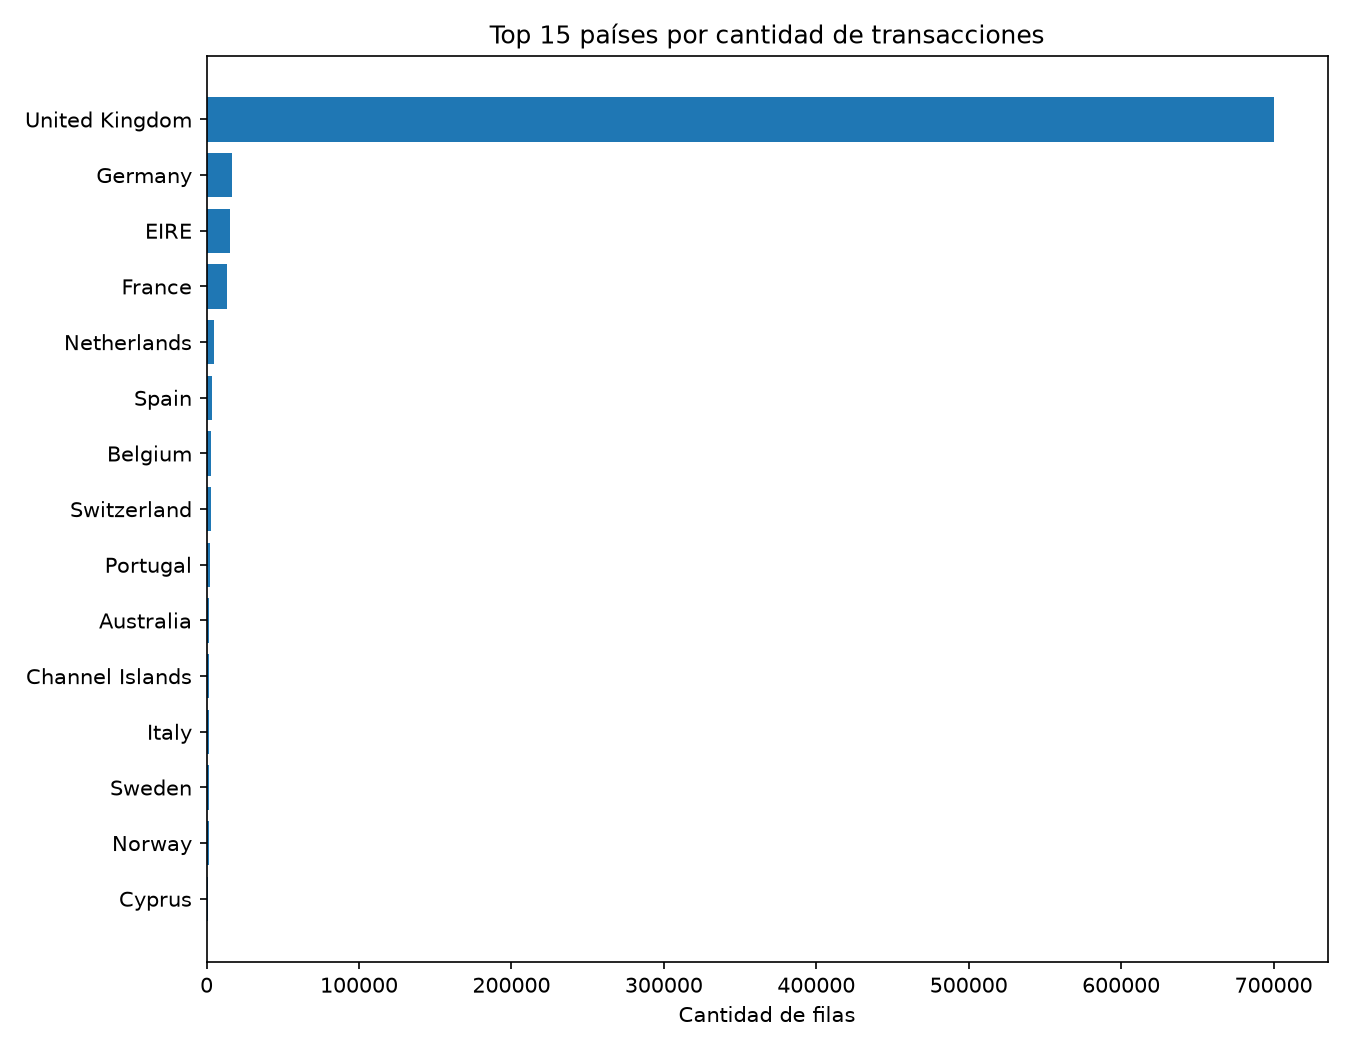
\includegraphics[width=0.8\textwidth]{../graficos/barras_paises.png}
	\caption{Top 15 países por cantidad de transacciones}
	\label{fig:barras-paises}
\end{figure}

\begin{figure}[h]
	\centering
	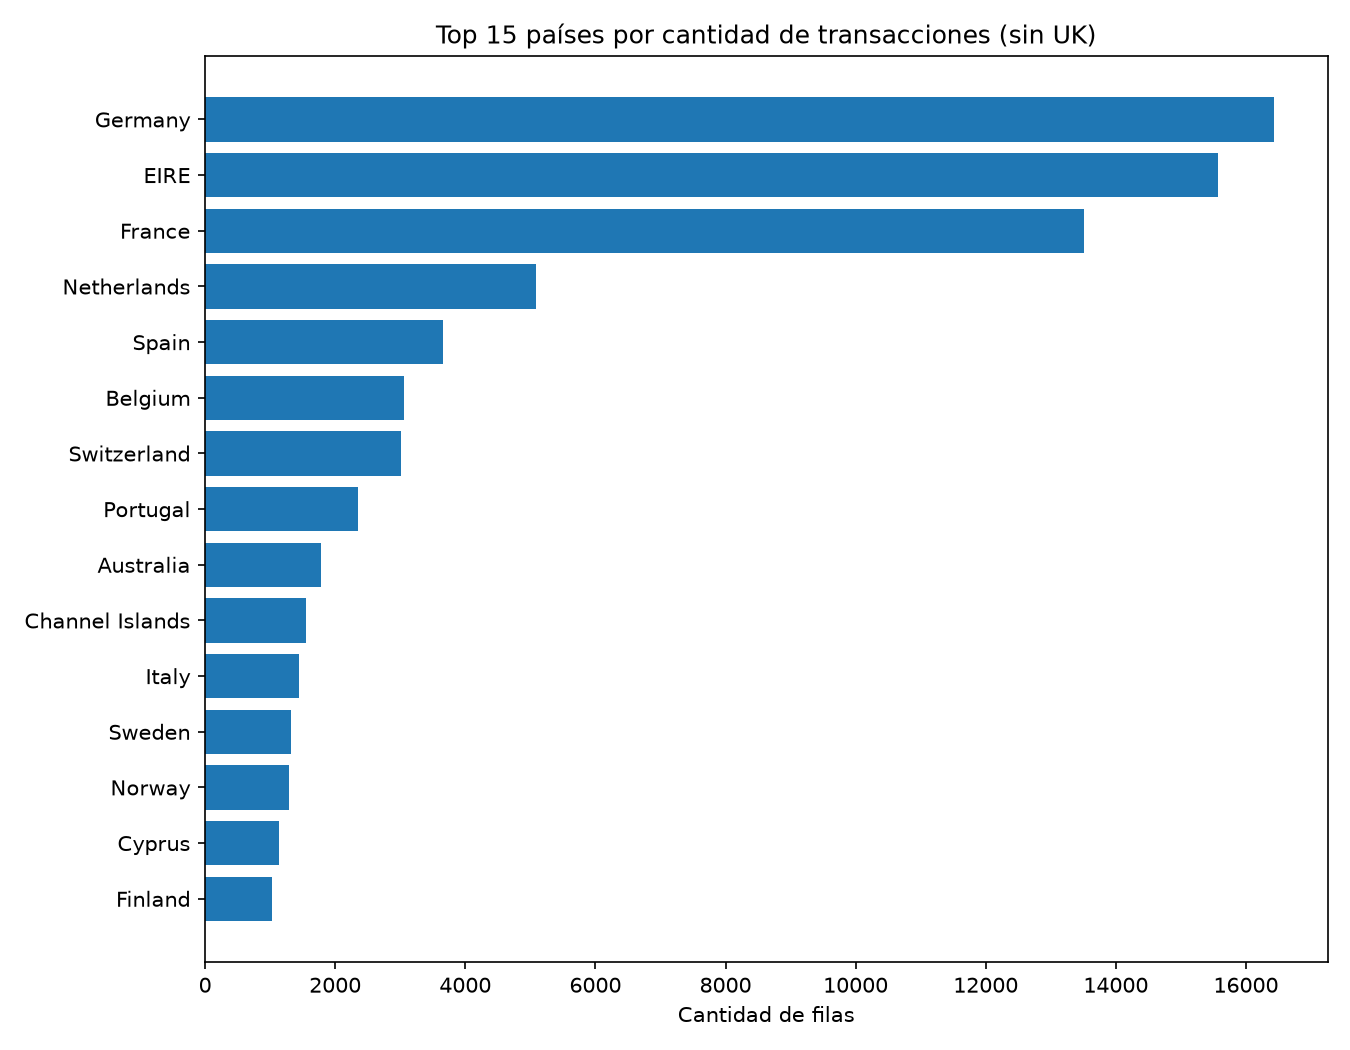
\includegraphics[width=0.8\textwidth]{../graficos/barras_paises_sin_uk.png}
	\caption{Top 15 países por cantidad de transacciones (excluyendo United Kingdom)}
	\label{fig:barras-paises-sin-uk}
\end{figure}


\subsection{Comparación de comportamiento entre países}

Para profundizar en el comportamiento de los clientes en los diferentes países, se compararon pares de países, calculando para cada uno: cantidad de filas, facturas únicas, clientes únicos, importe promedio, cantidad promedio, precio promedio, ticket promedio por factura, e ítems promedio por factura.

\begin{table}[h]
	\centering
	\caption{Comparación: United Kingdom vs. Lithuania}
	\label{tab:uk-lithuania}
	\begin{tabular}{lrr}
		\toprule
		& United Kingdom & Lithuania \\
		\midrule
		Filas                          & 700{,}388 & 154 \\
		Facturas únicas                & 33{,}541  & 6 \\
		Clientes únicos                & 5{,}350   & 1 \\
		Importe promedio (por línea)   & 20.54     & 31.77 \\
		Cantidad promedio (por línea)  & 12.18     & 14.97 \\
		Precio promedio                & 3.07      & 2.56 \\
		Ticket promedio por factura    & 429.00    & 815.45 \\
		Ítems promedio por factura     & 254.39    & 384.33 \\
		\bottomrule
	\end{tabular}
\end{table}

\begin{table}[h]
	\centering
	\caption{Comparación: France vs. Germany}
	\label{tab:france-germany}
	\begin{tabular}{lrr}
		\toprule
		& France & Germany \\
		\midrule
		Filas                          & 13{,}511 & 16{,}432 \\
		Facturas únicas                & 614      & 789 \\
		Clientes únicos                & 95       & 107 \\
		Importe promedio (por línea)   & 25.81    & 25.87 \\
		Cantidad promedio (por línea)  & 20.01    & 13.70 \\
		Precio promedio                & 4.29     & 3.59 \\
		Ticket promedio por factura    & 568.03   & 538.68 \\
		Ítems promedio por factura     & 440.21   & 285.37 \\
		\bottomrule
	\end{tabular}
\end{table}

\begin{table}[h]
	\centering
	\caption{Comparación: United Arab Emirates vs. Portugal}
	\label{tab:emirates-portugal}
	\begin{tabular}{lrr}
		\toprule
		& United Arab Emirates & Portugal \\
		\midrule
		Filas                          & 383     & 2{,}356 \\
		Facturas únicas                & 11      & 93 \\
		Clientes únicos                & 4      & 24 \\
		Importe promedio (por línea)   & 24.03   & 23.58 \\
		Cantidad promedio (por línea)  & 15.25   & 11.64 \\
		Precio promedio                & 3.64   & 5.10 \\
		Ticket promedio por factura    & 836.61  & 597.36 \\
		Ítems promedio por factura     & 530.82  & 294.87 \\
		\bottomrule
	\end{tabular}
\end{table}

\begin{table}[h]
	\centering
	\caption{Comparación: Netherlands vs. Germany}
	\label{tab:netherlands-germany}
	\begin{tabular}{lrr}
		\toprule
		& Netherlands & Germany \\
		\midrule
		Filas                          & 5{,}085  & 16{,}432 \\
		Facturas únicas                & 228      & 789 \\
		Clientes únicos                & 22       & 107 \\
		Importe promedio (por línea)   & 108.96   & 25.87 \\
		Cantidad promedio (por línea)  & 75.49    & 13.70 \\
		Precio promedio                & 2.69     & 3.59 \\
		Ticket promedio por factura    & 2{,}429.99 & 538.68 \\
		Ítems promedio por factura     & 1{,}683.68 & 285.37 \\
		\bottomrule
	\end{tabular}
\end{table}

\begin{table}[h]
	\centering
	\caption{Comparación: Japan vs. Switzerland}
	\label{tab:japan-switzerland}
	\begin{tabular}{lrr}
		\toprule
		& Japan & Switzerland \\
		\midrule
		Filas                          & 468    & 3{,}005 \\
		Facturas únicas                & 33     & 90 \\
		Clientes únicos                & 10     & 22 \\
		Importe promedio (por línea)   & 91.93  & 33.30 \\
		Cantidad promedio (por línea)  & 67.61  & 17.38 \\
		Precio promedio                & 2.01   & 3.82 \\
		Ticket promedio por factura    & 1{,}303.75 & 1{,}111.80 \\
		Ítems promedio por factura     & 958.88 & 580.30 \\
		\bottomrule
	\end{tabular}
\end{table}

\begin{table}[h]
	\centering
	\caption{Comparación: United Kingdom vs. Resto del mundo}
	\label{tab:uk-resto}
	\begin{tabular}{lrr}
		\toprule
		& United Kingdom & Resto del mundo \\
		\midrule
		Filas                          & 700{,}388 & 79{,}037 \\
		Facturas únicas                & 33{,}541  & 3{,}428 \\
		Clientes únicos                & 5{,}350   & 529 \\
		Importe promedio (por línea)   & 20.54     & 37.77 \\
		Cantidad promedio (por línea)  & 12.18     & 25.07 \\
		Precio promedio                & 3.07      & 4.57 \\
		Ticket promedio por factura    & 429.00    & 870.94 \\
		Ítems promedio por factura     & 254.39    & 578.05 \\
		\bottomrule
	\end{tabular}
\end{table}

\subsection{Discusión de resultados}

Las comparaciones muestran un patrón que se repite en la mayoría de los pares de países analizados: los países con menos clientes ytransacciones tienen un ticket promedio por factura más alto que aquellos que tienen más cantidad de clientes y transacciones. El caso más marcado es el de  Netherlands frente a Germany (Tabla~\ref{tab:netherlands-germany}): con menos de un tercio de las filas (5{,}085 frente a 16{,}432), Netherlands tiene un ticket promedio 4.5 veces mayor (2{,}429.99 contra 538.68). Se ve un patrón parecido, aunque menos marcado, entre Japan y Switzerland (Tabla~\ref{tab:japan-switzerland}) y entre United Kingdom y Lithuania (Tabla~\ref{tab:uk-lithuania}).

En el caso de France y Germany (Tabla~\ref{tab:france-germany}): ambos países tienen una cantidad de filas y facturas similarares entre sí (a diferencia de los pares anteriores, donde uno de los dos era claramente más chico). Consistente con el patrón general, sus valores de ticket promedio e importe promedio por ítem también son parecidos entre sí, lo que refuerza la idea de que la diferencia de ticket promedio está más asociada al volumen relativo de cada país que a otro factor.

La comparación entre United Arab Emirates y Portugal (Tabla~\ref{tab:emirates-portugal}) refuerza el mismo patrón: aunque United Arab Emirates tiene muchas menos filas, facturas y clientes que Portugal, su ticket promedio por factura es más alto (836.61 frente a 597.36) y tiene casi el doble de ítems promedio por factura (530.82 frente a 294.87).

La comparación más interesante es la de United Kingdom contra el resto del mundo (Tabla~\ref{tab:uk-resto}). United Kingdom concentra el 89.86\% de las transacciones, pero el resto del mundo tiene un ticket promedio por factura de 870.94, más del doble que United Kingdom (429.00), y también más ítems promedio por factura (578.05 frente a 254.39). Esto sugiere que los clientes fuera de Reino Unido tienen, en promedio, un perfil de compra más parecido al de un mayorista o distribuidor, mientras que dentro de Reino Unido el comportamiento se parece más al de un consumidor minorista.



\end{document}